\chapter[Description]{Description of program}
\label{chap:description}

\section{Program structure}
The developed application is devided into three modules.
\begin{itemize}
\item Conversion
\item LCD
\item uip
\end{itemize}
\begin{center}
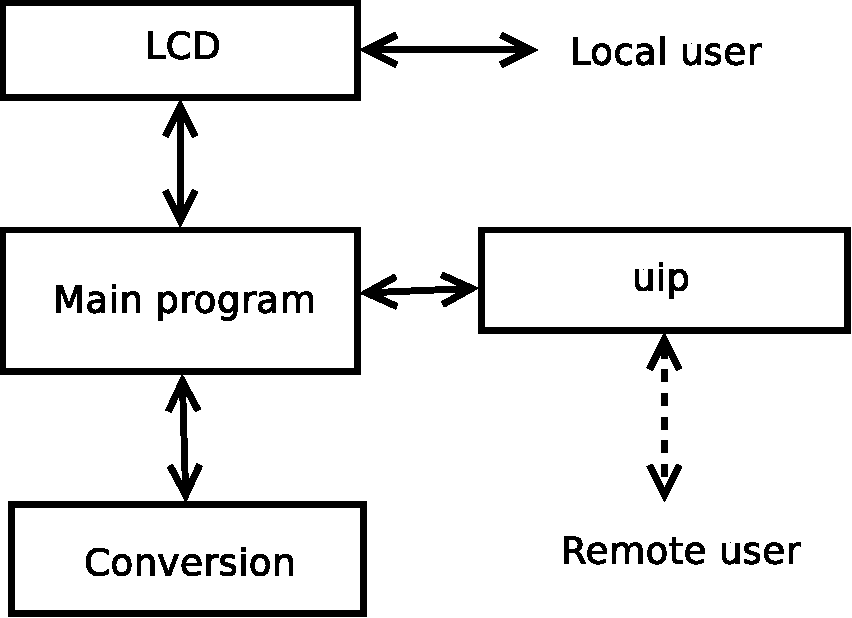
\includegraphics[scale=0.4]{figs/program_structure.pdf}
\end{center}

The conversion part is responsible for most of the ADC, DAC, GPIO and interrupt handling parts of the program. The LCD is taking care of the physical user interface, both touchscreen and displaying values on the screen. The uip is accepting remote connections and serving data to remote clients.\\\\
The program runs roughly this sequence:
\begin{center}
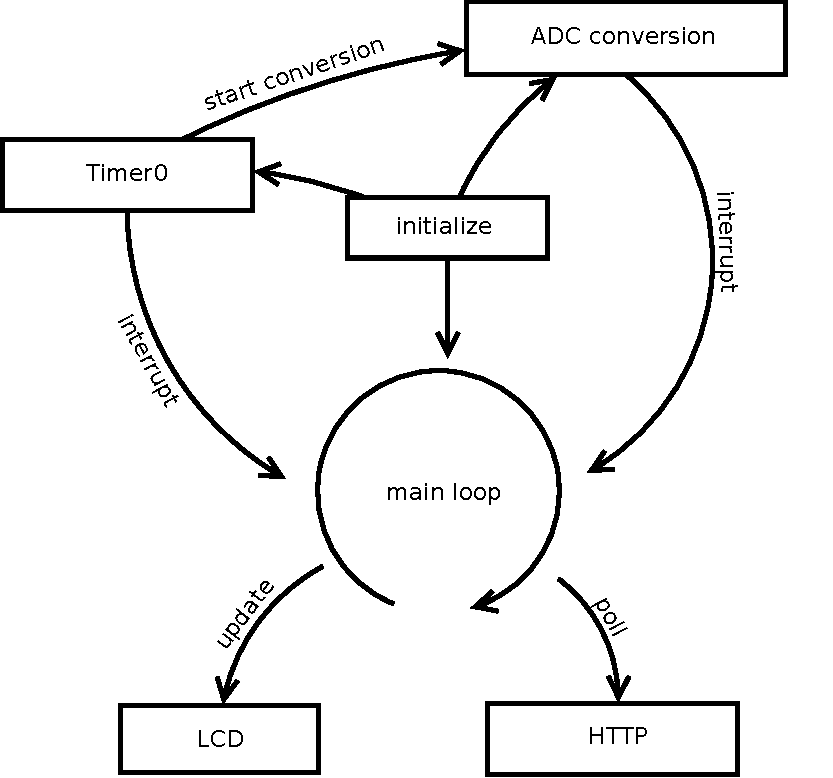
\includegraphics[scale=0.4]{figs/program_sequence.pdf}
\end{center}
The first thing done is the initialization. This obviously only run once. It gets the interrupts up and running and configures the appropriate GPIO pins. When done, it enters the main loop, where the application remains for remainder of run-time, while not processing interrupts. The Timer0 runs at a predefined frequency, and takes care of [INSERT TEXT]\\\\

The ADC interrupt takes care of [INSERT TEXT].\\\\
When not doing interrupts the main loop updates the screen, checks if a user has touched the screen and moves the cursor accordingly.\\
It also does periodic checks on the IP stack, sending and recieving packets at a resonably stable frequency. This is done via the HTTP server.
\section{Measurements and control}
\subsection{Hardware resource allocation}
\subsubsection{ADC}
We are using the ADC for two purposes: Detecting input from the touchscreen and measuring grid frequency. This takes up three channels (one for each dimension on the screen, and one dedicated to the frequency). To get the maximum number of samples per second, we use burst mode. \\
\begin{center}
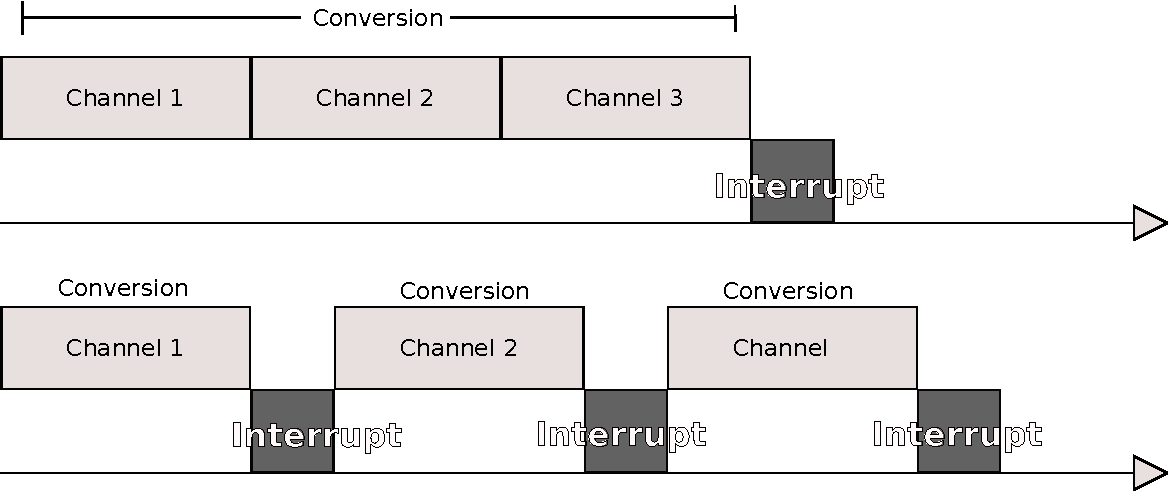
\includegraphics[scale=0.5]{figs/burst_mode.pdf}
\end{center}
Burst is started by entering Timer0 interrupt
% explanation of burst mode, timer0 and ADC conversion timer. Graphic picturing burst mode





\subsection{Measurement algorithms and their implementation}
The values measured with the microcontroller (ADC) are:
\begin{itemize}
\item Grid frequency
\item Grid voltage
\item Grid current
\item LCD voltege (checking if, and if yes then where, LCD screen has been touched)
\end{itemize}

\subsubsection{Voltage and Current measurements}
The voltage from the grid had to be passed through a circuit that would lower it's value to 0...3.3V range, before it could be processed by the microcontroller. The same thing had to be done with the current - it had to be converted to a voltage signal of the same scope. Both signals were scaled afterwards so the output of calculations would be in grid values. Two different approaches were used for each of them.

\paragraph{Voltage scaling}
Firs the RMS and offset values of the grid voltage has been measured. The results were: 
\[ V_{RMS}=236V \] 
\[ V_{Offset} \approx 0V\]
We can conver them into peak-to-peak values:
\[ V_{p-p}=2(V_{RMS}-V_{Offset})\sqrt{2}=2(236V-0)\sqrt{2}=667.5V \]
Since the offset is approximately zero we can wrtie that maximum an minimum values of volatege are $ \pm333.75V $. The maximum and minimum quantization levels accuired by ADC conversions were 1002 and 20. Hence the zero Volts was represented by $ (1002-20)/2=491_{levels} $ and $ 1_{level}=333.75_{volts}/491_{levels}=0.679735234_{volts} $.

\paragraph{Current scaling}
A bit different approach have been used while calculating the scaling ratio in the case of the grid's current. Here we've assumed that the current converting circuit is very precise and that the output values are exactly 0....3.3V. Thus we can suspect that the amount of bits corresponding to 0A is equal to 512. After aquring the raw samples of the measured current from ADC, substracting 512, calculating their RMS value and multiplying the result by $ \sqrt{2} $ we get the current signal's digital representation's amplitude, which represents the real signals amplitude. Sclaing is done as in the case of the voltege from this point.

\subsubsection{Frequency measurement}
The frequency measurement is done by calculating the length of the period of a given signal. We've done this by calculating the number of samples between the points at wich the signal is crossing an arbitrairly defined zero line with an assumed direction (rising edge or falling edge) and comparing it (number of samples) with the sampling frequency.\\
In order to detect zero-crossing two succeding samples had to be remembered by the system. If the previous sample was below the zero-level and the current one is above, than the system marks this time as a rising edge zero-crossing and starts to count the samples until the next one.\\
Due to significant disturbances a low pass filter had to be used, in order to smoothen out the data. Without it detecting false zero-crossings would be very common, which in turn would render the method completly useless.\\
The lowpass filter is used only for this particular purouse, though. All the other calculations, like voltage RMS value, power etc. were performed on raw data.

\subsubsection{LCD measurements}
The LCD measurements are conducted to check if the touch screen has been touched and if yes, where exactly did it happen. The possition of the touch is determined by measuring the voltage on the LCD's outputs. Measurement of the X and Y coordinates arn't done simultanously. If we want to measure the X coordinate the ADC and the pins have to be set to a certain state. In order to meassure the Y coordinate those set up options have to be different. Hence, every coordinate is meassured on every second ADC action.

 
\section{User interface}
\section{Communication}
The communication part of the program is done by reusing the uip network stack. The built-in http server has the ability to both serve files and do some basic server-side scripting. \\
We plan on refactoring the server, making able to serve xml and xsl\footnote{XML Stylesheet} (with the right content-type). Xsl will enable us to generate a single xml file and then transform it for the user to view via a browser. The xml document will be treated as a regulear html page, making the transformation transparent for the user. \\
The really nice thing about xsl is that we only need one source of information for both the userinterface (webpage) and for automatically downloading done by programs interested in only the data. The programs will disreguard the xml stylesheet and only fetch the data, minimizing overhead.
\subsection{Implementation}
The first step in getting the webserver working as we intended was getting the stand-alone server accepting xml files. This was relatively easy, and do was getting the server to generate content dynamically. This was mostly done by copy-pasting, so we wont bore you with the details - the code is included.\\
The next step was getting the generic server merged into our main project. The big challenge was that the uip server used a global timer, and not just any timer - the same timer we already used i our main project.\\
The migration was again done in two steps. First step was moving the httpd timer from timer0 to timer1, and check if that worked. Next step was merging the code of the two timers into one, and get the timing right. The change from timer0 to timer1 resulted in a very slow, but working, webserver.\\\\
The problem in merging the two timers was due to the fact that they ran at two different frequencies. One at 20MHz and another at 100Hz. As these was both defined in our config.h as respectively TIMER0\_TICK\_PER\_SEC and HTTPD\_TICK\_PER\_SEC we figured we needed to add a counter and do the following:
\begin{equation}
  counter \% \frac{TIMER0\_TICK\_PER\_SEC}{HTTPD\_TICK\_PER\_SEC} = 0
\end{equation}
The \% is the modulus operation. Upon true, the counter should reset and the http tick should increment. This implementation should make the http server insensible to changes in the timer0 frequency.\\\\
The webpage itself refreshes every 5 seconds by asking the browser to do a delayed redirect to the same page.

\subsubsection{Historical values}
Although not implemented, due to different focus, we have spent some time considering a possible implementation.\\
At first glance the buffer could be implemented using a linked list - but due to the fact that we do not have at memory manager we would at some point run out of free memory to store these these historical values. So, we could use a fixed size array of int pointers, and a pointer to the last element inserted. Then it should be possible to run through the array ``array-size'' number of times, starting from ``last\_inserted'' and break if we encounter a null pointer.\\
The historical values should be displayed on a graph generated as an svg image, using JQuery to reload the values.

\section{Chapter Summary}
\label{sec:SummaryDescription}
\subsection{Communication}
The finished result can be viewed by accessing the ip (typically 192.168.0.100) and requesting the data.xml document. When doing this from a browser the transformation works like a charma and gives us a graphical representation of our values. The server is still slow when we enable the LCD and touchscreen, but this should just a matter of opimizing the code that handles these.\\
The xsl file is with the other files in the uip/http-fs folder. 
